\section{Limits}
\subsection{Introduction to Limits}
Limits form the very backbone of calculus, almost every concept and definition comes from the limit of something else. Intuitively they are quite simple: the limit of a something is simply where is appears to be going. In practice, we need a much more rigorous definition. To see why, we turn to the ancient Greeks.

In around 450 BC, Zeno, as ancient Greek philosophers tended to do, sat around thinking of paradoxes. Here are two of his most famous:
\begin{enumerate}
	\item \href{https://en.wikipedia.org/wiki/Atalanta}{Atalanta}\footnote{Famous figure in Greek mythology} is trying to walk to the end of a path. To walk the entire path she must first walk half the path, then half the remaining path (a quarter), then half the next remaining path (an eigth), then a sixteenth, a thirty-second, etc. Since Atalanta has to walk an infinite number of paths, how can she ever finish walking the path? 
	\item \href{https://en.wikipedia.org/wiki/Achilles}{Achilles}\footnote{Even more famous figure in Greek mythology} is racing a \href{https://en.wikipedia.org/wiki/The_Tortoise_and_the_Hare}{tortoise}\footnote{A very famous figure in fairy tale lore, famously starred in the hit movie ``Tortoise and the Hare"}. To make if fair, he gives the tortoise a head start (say 100m). Once he takes off and covers the first 100m, the tortoise would've meandered a couple more meters. Once he runs the next few meters, the tortoise will cover a few more meters, and so on so forth. So the questions is: If every time Achilles catches up to where the tortoise was prior, the tortoise remains a bit ahead, how will Achilles ever pass the tortoise?
\end{enumerate}

The astute reader may notice that these paradoxes are clearly resolvable. After all, we walk across paths all the time and obviously Achilles will eventually pass the turtle, so why are these so famous? 

The reason why these paradoxes are even talked about now is because they deal with the concept of infinity and infinitesimals (infinitely small distances). In order to have a precise mathematical way of dealing with these, we must invent new mathematics. That new mathematics is Calculus.

To introduce the idea of a limit, let's write the Atalanta (formally known as the Dichotomy) paradox in terms of limits (kind of). For Atalanta, suppose the path is 1m long and she walks at a speed of 1m/s. Then the time taken will be
\[ t = \frac{1}{2} + \frac{1}{4} + \frac{1}{8} + \frac{1}{16} + \cdots \]

Let's try to add up the terms in this sequence, if $n$ is the number of terms we add up
\begin{center}
\begin{tabular}{|c|c|c|c|c|c|c|c|c|c|}
\hline 
n & 1 & 2 & 3 & 4 & 5 & $\cdots$ & 10 & $\cdots$ & $\infty$ \\ 
\hline 
t & 1/2 & 3/4 & 7/8 & 15/16 & 31/32 & $\cdots$ & 1023/1024 & $\cdots$ & 1 \\ 
\hline 
\end{tabular} 
\end{center}

We see that as $n$ gets really, really large, then $t$ gets really close to 1. This makes sense because Atalanta should be able to walk the 1m path in 1s.

With that history lesson out of the way, let's return to the math. Take a simple function, for instance $f(x) = x$, and let's look at how it behaves around $x = 1$. There's two ways we can answer this question:
\begin{enumerate}
	\item Start from the left of the graph and see what happens as we move up to $x = 1$
	\item Start from the right of the graph and see what happens as we move down to $x = 1$
\end{enumerate}

It's pretty obvious in this case, but we see that the graph approaches $y = 1$ regardless of which direction we approach. This idea of seeing what happens when we get close to a value is formalized in the definition of a limit.

\begin{definition}[The Limit]
Let $f(x)$ be a function and $a, L$ some real numbers. If all values of $f(x)$ approach $L$ as $x$ approaches $a$, then we say that $L$ is the limit of the function $f(x)$ as $x$ approaches $a$. In symbols, we write this as
\[ \lim_{x \to a} f(x) = L \]
\end{definition}

\begin{example}
What we got from the previous simple example is that
\[ \lim_{x \to 1} x = 1 \]
\end{example}

A quick and dirty way to evaluate limits is to evaluate a bunch of values progressively closer to the value we wish to look at. If the $y$ values appears to get closer to some number, then that number is probably the limit.

\begin{example}

Consider the function $f(x) = x^2$ and suppose we want to find the limit as $x$ approaches $2$. To evaluate this limit using a table, we compute the following values:

\begin{center}
\begin{tabular}{|c|c|c|c|c|c|c|}
\hline 
x & 1.9 & 1.99 & 1.999 & 2.001 & 2.01 & 2.1 \\ 
\hline 
f(x) & 3.61 & 3.9601 & 3.996001 & 4.004001 & 4.0401 & 4.41 \\ 
\hline 
\end{tabular} 
\end{center}

From looking at this table, we can make an educated guess at the limit
\[ \lim_{x \to 2} x^2 = 4 \]

\end{example}

The method of evaluating limits using a table is very crude and, as we saw, very difficult without some form of computer assistance. Throughout mathematics, it is most common to evaluate limits algebraically. First, we discuss the notion of a one-sided limit.

\newpage 
\begin{definition}[One-Sided Limits]
Let $f(x)$ be a function and $a$ some real number. There are two different one-sided limits:
\begin{itemize}
	\item If $f(x)$ approaches a real number $L$ as $x$, where $x < a$, approaches $a$, then the \textbf{left-sided limit} of $f(x)$ as $x$ approaches $a$ is $L$, or in symbols
	\[ \lim_{x \to a^-} f(x) = L \]
	\item If $f(x)$ approaches a real number $M$ as $x$, where $x > a$, approaches $a$, then the \textbf{right-sided limit} of $f(x)$ as $x$ approaches $a$ is $M$, or in symbols
	\[ \lim_{x \to a^+} f(x) = M \]
\end{itemize}
\end{definition}

\begin{example}
Consider a piecewise function
\[ f(x) = \begin{cases} 
x & x \leq 0 \\
x^2 + 1 & x > 0
\end{cases} \]

If we approach 0 from the left, we are on the top function. We can plug in 0 directly to find
\[ \lim_{x \to 0^-} f(x) = 0 \]

From the right we are on the bottom function. We can still plug in 0 even though the condition is $x > 0$ because limits are not about what the function actually is, rather it is about what the function is approaching. Thus
\[ \lim_{x \to 0^+} f(x) = 0^2 + 1 = 1 \]

\end{example}

This method of ``plug-and-chug" is generally how most limits will be evaluated. In the rare case that this doesn't work (for instance we end up dividing by zero), we'll need to do some more algebra.

\begin{theorem}[Two-Sided Limits]
The limit of a function $f(x)$ as $x$ approaches $a$ exists if and only if both one-sided limits exist and are equal, that is
\[ \lim_{x \to a} f(x) = \lim_{x \to a^-} f(x) = \lim_{x \to a^+} f(x) \]
\end{theorem}

Thus we cannot conclude that a limit exists unless both the left- and right-handed limits exist and are equal. 

\begin{example}
	Let $a$ and $c$ be any two real numbers, the two most basic limits are
	\[ \lim_{x \to a} c = c \qquad \lim_{x \to a} x = a \]
\end{example}


\begin{example}
	Sometimes the limit does not exist because we try to do something illegal, for instance
	\[ \lim_{x \to -4} \sqrt{x} = \varnothing \]
	because we cannot square root a negative\footnote{Technically we can, but then we would have to work in the complex plane and that requires much more complicated machinery (complex analysis)}
\end{example}

\begin{example}
	Consider a piecewise function
	\[ f(x) = \begin{cases} 
	\sin(x) & x \leq 0 \\ 
	\cos(x) & x > 0 
	\end{cases} \]
	We have the following one-sided limits
	\[ \lim_{x \to 0^-} f(x) = 0 \qquad \lim_{x \to 0^+} f(x)= 1 \]
	Since the two are not equal, the limit of $f(x)$ as $x$ approaches $0$ does not exist.
\end{example}

Sometimes we end up trying to do something illegal when we ``plug-and-chug," but that does not always mean the limit doesn't exist. In some cases infinity (or negative infinity) is a perfectly valid answer\footnote{Though it can be debated if these limits actually exist}. Identifying infinite limits requires a bit of brainpower. The process is similar to making a table of values but we don't actually do it. It's easiest to demonstrate with examples:

\begin{example}
	Consider the function $f(x) = 1/x$ as $x$ approaches 0. From the right side we get smaller and smaller $x$ values, which means that $f(x)$ gets larger and larger. Thus we can write
	\[ \lim_{x \to 0^+} f(x) = \infty \]
	From the left side we also get smaller and smaller values, but negative. Thus rather than get bigger, $f(x)$ gets more and more negative, so we write
	\[ \lim_{x \to 0^-} f(x) = -\infty \]
	Since these two one-sided limits are not the same, the limit does not exist.
\end{example}

\begin{example}
	Now consider the function $f(x) = 1/x^2$. We can use a similar argument from last time, but since the denominator is squared, the function will always be positive. Thus
	\[ \lim_{x \to 0} f(x) = \lim_{x \to 0^-} f(x) = \lim_{x \to 0^+} f(x) = \infty \]
\end{example}

The value of the limit is not the only place where infinity could exist, we may be interested in the behavior of the function as $x$ itself approach positive/negative infinity. Again, we demonstrate with an example:

\begin{example}
	Consider the function $f(x) = 1/x$ again. Suppose we want to know the limit as $x$ goes to infinity. To do this, we think about what happens as $x$ gets larger and larger. Clearly $f(x)$ would get smaller and smaller as the denominator grows, so
	\[ \lim_{x \to \infty} f(x) = 0 \]
	Similarly, we can show that
	\[ \lim_{x \to -\infty} f(x) = 0 \]
\end{example}

Limits with infinity gives us a way to find asymptotes without having to draw a graph.
\begin{theorem}[Asymptotes]
	Let $f(x)$ be a function and $a$ a real number. The line $x = a$ is a vertical asymptote if both one-sided limits are positive or negative infinity. In symbols
	\[ \lim_{x \to a^-} f(x) = \pm \infty \qquad \lim_{x \to a^+} f(x) = \pm \infty \]
	Note that this does not mean the limit itself is defined as we say in the case of $f(x) = 1/x$. 
	
	The line $y = a$ is a horizontal asymptote if the limit as $x$ goes to positive or negative infinity is $a$.
	\[ \lim_{x \to -\infty} f(x) = a \qquad \text{ or } \qquad \lim_{x \to \infty} f(x) = a \]
\end{theorem}

\begin{example}
	Let's find all asymptotes for the following function
	\[ f(x) = \frac{1}{1 - x} + 3 \]
	First we do the horizontal asymptotes
	\[ \lim_{x \to -\infty} f(x) = \lim_{x \to \infty} f(x) = 3 \]
	so $y = 3$ is a horizontal asymptote for this function.
	
	It's a bit harder to see the vertical asymptotes right away, but a good way to find them is to look for ``divide by zeros" and then evaluate the limits. In this case we consider $x = 1$
	\[ \lim_{x \to 1^-} = \infty \qquad \lim_{x \to 1^+} = - \infty \]
	Notice that the left handed limit is positive infinity this time. This is because when $x < 1$, the denominator is very small but positive. When dealing with infinities, it is very important to make sure you have the right one.
\end{example}

If we are given a graph of a function, we can evaluate limits visually by examining the behavior of the graph. For instance if we wanted to evaluate a left-handed limit, we can place our pencil a bit to the left of the point and trace the line up to that point. The height that we appear to be approaching is the limit. Remember: the limit is what the function appears to approaching, not what it actually is.\footnote{If it helps, you may think of limits as "It is not the destination that matters, but the journey"}

\begin{example} 
Consider the following graph of a function $f(x)$
\begin{center}
	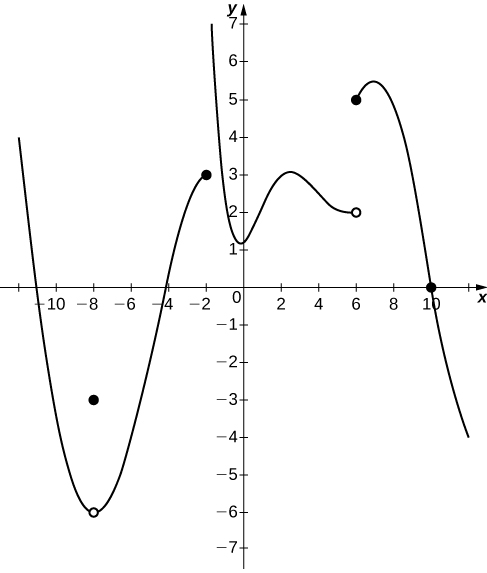
\includegraphics[scale=1]{images/Figure 2.2.1.jpg}
\end{center}

At $x = -8$, we see that from the left and the right we are approaching the same value. The fact that $f(-8) = -3$ does not matter, the limits are
\[ \lim_{x \to -8^-} f(x) = \lim_{x \to -8^+} f(x) = \lim_{x \to -8} f(x) = -6 \]

At $x = -2$ the graph has different behavior depending on if we are on the left or right. If we trace the graph coming from the left, we will approach $y = -2$ and in fact this is also the value of $f(-2)$. If we come from the right then we go straight up to $+ \infty$. Thus
\[ \lim_{x \to -2^-} f(x) = 3 \qquad \lim_{x \to -2^+} = \infty \qquad \lim_{x \to -2} = \varnothing \]

The remaining two interesting points, $x = 6$ and $x = 10$, will be left as an exercise to the sufficiently motivated and astute reader.
\end{example}

\newpage 
\subsection{Techniques for Limits}

Now that we've brute forced our way through a couple limits, it is time to find a way to use those previous results to evaluate new limits. A lot of these laws/rules may seem obvious but it is important to state them nonetheless.

\begin{theorem}[Properties of Limits]
	Let $f(x)$ and $g(x)$ be functions, $a$ a real number, and suppose $f,g$ have the following limits
	\[ \lim_{x \to a} f(x) = L \qquad \lim_{x \to a} g(x) = M \]
	
	Then we have the following properties, let $c$ be a constant
	\begin{align*}
		\lim_{x \to a} f(x) \pm g(x) &= \lim_{x \to a} f(x) \pm \lim_{x \to a} g(x) = L \pm M \\
		\lim_{x \to a} f(x)g(x) &= \lim_{x \to a} f(x) \cdot \lim_{x \to a} g(x) = L \cdot M \\
		\lim_{x \to a} cf(x) &= c \cdot \lim_{x \to a} f(x) = c \cdot L \\
		\lim_{x \to a} \frac{f(x)}{g(x)} &= \frac{\lim_{x \to a} f(x)}{\lim_{x \to a} g(x)} = \frac{L}{M} \qquad \text{ if $M \neq 0$} \\
		\lim_{x \to a} (f(x))^n &= \qty(\lim_{x \to a} f(x))^n = L^n \\
		\lim_{x \to a} \sqrt[n]{f(x)} &= \sqrt[n]{\lim_{x \to a} f(x)} = \sqrt[n]{L}
	\end{align*}
	
	The last result holds for all $x$ if $n$ is odd and all $x \geq 0$ if $n$ is even (these also happen to be the domains of $\sqrt[n]{x}$ for odd/even $n$).
\end{theorem}

These laws give the ``plug and chug" strategy a more mathematical reasoning. Since we know the two basic limits
\[ \lim_{x \to a} c = c \qquad \lim_{x \to a} x = a \]
we can use the limit laws to manipulate them into the function we are interested in. 

\begin{example}
	Consider the function
	\[ f(x) = \frac{x^2 + 3x - 10}{x^3 - 2x} \]
	
	The using the basic limits, we can evaluate the limit
	\[ \lim_{x \to 2} f(x) = \frac{2^2 + 3 \cdot 2 - 10}{2^3 - 2 \cdot 2} = \frac{0}{4} = 0 \]
\end{example}

It is worth noting that these laws all apply the one-sided limits as well.

There are many tricks to evaluating limits, we'll cover a few of the most common ones in the ensuing exercises.
\begin{example}
	Consider the function
	\[ f(x) = \frac{x^2 + 2x - 3}{x^2 - 1} \]
	
	If we tried to evaluate the limit as $x$ approaches 1, then we would end up dividing by zero. To avoid this we must first factor the top and bottom
	\[ f(x) = \frac{(x + 3)(x - 1)}{(x + 1)(x - 1)} = \frac{x + 3}{x + 1} \]
	Now we see that since a term cancels, we can use the limit laws to evaluate
	\[ \lim_{x \to 1} f(x) = \frac{1 + 3}{1 + 1} = 2 \]
\end{example}

\begin{example}
	When working with square roots it is common to get a function of the form
	\[ f(x) = \frac{\sqrt{x + 1} - 1}{x} \]
	
	If we tried to evaluate the limit as $x$ approaches 0 it would appear to seem that we are stuck. Furthermore there is nothing to factor, so what is there left to do? It turns out that we can use the fact that $x^2 - a^2 = (x + a)(x - a)$ change the fraction. This is known as multiplying by the conjugate, lets see it in action:
	\begin{align*}
		f(x) &= \frac{\sqrt{x + 1} - 1}{x} \cdot \qty(\frac{\sqrt{x + 1} + 1}{\sqrt{x + 1} + 1}) = \frac{(\sqrt{x + 1})^2 - 1^2}{x(\sqrt{x + 1} + 1)} \\
		&= \frac{x + 1 - 1}{x(\sqrt{x + 1} + 1)} = \frac{x}{x(\sqrt{x + 1} + 1)}\\
		&= \frac{1}{\sqrt{x + 1} + 1}
	\end{align*}
	
	This sort of algebraic manipulation is allowed because at the end of the day, all we did was multiply by 1. With the function in this form, we can now evaluate the limit
	\[ \lim_{x \to 0} f(x) = \frac{1}{\sqrt{0 + 1} + 1} = \frac{1}{2} \]
\end{example}

\begin{example}
	When evaluating limits, one should always try to simplify the function as much as possible before preceding. Consider the function
	\[ f(x) = \frac{1}{x} - \frac{3}{x(x + 3)} \]
	
	If we tried to evaluate the limit as $x$ goes to 0, we may be tempted to either say it does not exist or is an asymptote due to the $1/x$. But if we took the time to simply, we find
	\[ f(x) = \frac{x + 3}{x(x + 3)} - \frac{3}{x(x + 3)} = \frac{x}{x(x + 3)} = \frac{1}{x + 3} \]
	Now we can evaluate
	\[ \lim_{x \to 0} f(x) = \frac{1}{0 + 3} = \frac{1}{3} \]
\end{example}

For more complicated limits we may sometimes use the squeeze (or sandwich) theorem when applicable.
\begin{theorem}[Squeeze Theorem]
	Let $f(x), g(x), h(x)$ be functions defined for all $x \neq a$ in an open interval containing $a$. If
	\[ f(x) \leq g(x) \leq h(x) \]
	Then their limits obey
	\[ \lim_{x \to a} f(x) \leq \lim_{x \to a} g(x) \leq \lim_{x \to a} h(x) \]
	
	In particular if
	\[ \lim_{x \to a} f(x) = \lim_{x \to a} h(x) = L \]
	then it must be the case that
	\[ \lim_{x \to a} g(x) = L \]
\end{theorem}

To see how we may use this theorem to solve otherwise impossible limits, consider the following example.

\begin{example}
	Suppose we have a function
	\[ f(x) = x^2 \cos(\frac{1}{x}) \]
	and we wish to evaluate the limit as $x$ goes to 0. We can't use the limit laws because then we'd be dividing by zero, so instead we note that
	\[ -1 \leq \cos(x) \leq 1 \qquad \text{ and so } \qquad -x^2 \leq f(x) \leq x^2 \]
	
	It doesn't matter what's inside the cosine because it will always be between -1 and +1. Thus we just need to compute
	\[ \lim_{x \to 0} -x^2 = 0 \qquad \lim_{x \to 0} x^2 = 0 \]
	and we are able to conclude, using the squeeze theorem,
	\[ \lim_{x \to 0} f(x) = 0 \]
\end{example}

Note that in order to actually get a limit out of the squeeze theorem, the limit on both sides of the inequality must be the same. If they are different, then the squeeze limit does not tell us anything.

\begin{Optional}[Important Trigonometric Limits]
For this subsection I will use without proof the following limits\footnote{A geometric proof of the first limit using the squeeze theorem is provided in the textbook and the second can be found by multiplying by the conjugate}
\[ \lim_{x \to 0} \frac{\sin(x)}{x} = 1 \qquad \lim_{x \to 0} \frac{1 - \cos x}{x} = 0\]

Let's see how we can use these two limits to evaluate a deceptively difficult limit

\begin{example}
	Consider the function
	\[ f(x) = \frac{\sin^2(3x)}{\sin(2x)} \]
	
	We want to evaluate the limit as $x$ approaches $0	$. At first glance, we don't really see much that we can do. After all, both the numerator and denominator goes to zero. However, before we give up and quit math forever, we notice that there is one (indeed the only) thing to do: rewrite the numerator. 
	\[ f(x) = \frac{1 - \cos^2(3x)}{\sin(2x)} = \frac{(1 + \cos(3x))(1 - \cos(3x))}{\sin(2x)} \]
	
	We now remember that we've seen part of this numerator before, it's the same numerator in the limit we first introduced! But we're missing the denominator, furthermore the function instead the cosine is $x$, not $3x$. To fix this, we turn to the old trick: multiply by 1. This also fixes the sine in the denominator
	\begin{align*}
		f(x) &= \frac{(1 + \cos(3x))(1 - \cos(3x))}{\sin(2x)} \cdot \qty(\frac{2x}{2x}) \cdot \qty(\frac{3x}{3x}) \\
		&= \qty(\frac{2x}{\sin(2x)}) \cdot \qty(\frac{1 - \cos(3x)}{3x}) \cdot \qty(\frac{2x(1 + \cos(3x))}{3x}) \\
		&= \frac{2}{3} \qty(\frac{1}{\sin(2x)/2x}) \qty(\frac{1 - \cos(3x)}{3x}) (1 + \cos(3x))
	\end{align*}
	Now we can evaluate the limit
	\[ \lim_{x \to 0} f(x) = \frac{2}{3} \cdot \frac{1}{1} \cdot 0 \cdot (1 + 0) = 0 \]
\end{example}

\end{Optional}

\newpage 
\subsection{Continuity}

At its essence, a function is continuous if you can draw if without picking up your pencil. This means that functions like $x, x^2, \sin(x)$ are continuous while $1/x$ is not. However intuition is never good enough and we need a formal mathematical definition of what it means for a function to be continuous. First, we need to be able to visually tell when a function is discontinuous, this is easy:

% Add some pictures
There are three ways a function fails to be continuous
\begin{enumerate}
	\item A removable (or hole) discontinuity: there is a missing point, the function may or may not be defined there
	\item A jump discontinuity: the function literally jumps
	\item An infinite discontinuity: there is a vertical asymptote (think $1/x$)
\end{enumerate}

\begin{center}
	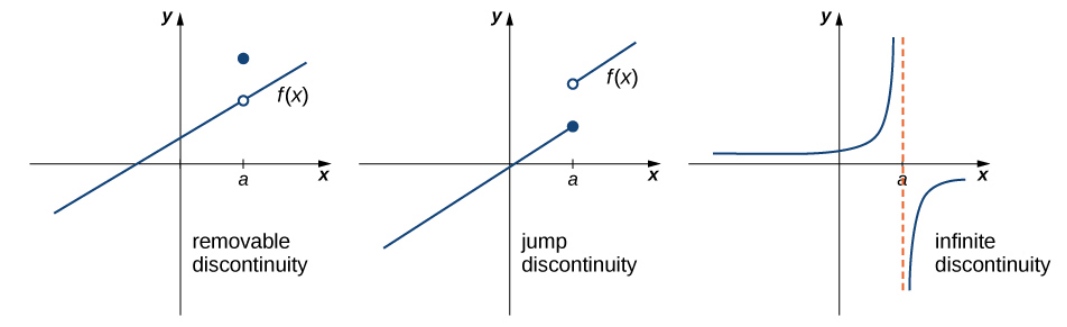
\includegraphics[scale=0.55]{images/Figure 2.3.1.png} 
\end{center}

Now that we know what it looks like when a function is not continuous, we can write down a definition. 
\begin{definition}
	A function $f(x)$ is continuous at a point $x = a$ if all of the following hold:
	\begin{itemize}
		\item The function is defined at $x = a$, that is $f(a)$ is defined
		\item The limit $\lim_{x \to a} f(x)$ exists
		\item The two above quantities are equal
		\[ \lim_{x \to a} f(x) = f(a) \]
	\end{itemize}
	We say that $f(x)$ is discontinuous at $x = a$ if any of the above fail.
\end{definition}

This definition captures the essence of ``not lifting up your pencil." Requiring that the function exist means that we won't have any infinite discontinuities and requiring it equal the limit means that there will not be any hole or jump discontinuities.

\begin{example}
	Suppose we have a piecewise function
	\[ f(x) = \begin{cases}
	\sin(x) \qquad x \leq 0 \\
	\cos(x) \qquad x > 0
	\end{cases} \]
	We have two limits as $x$ approaches 0
	\[ \lim_{x \to 0^-} f(x) = \sin(0) = 0 \qquad \lim_{x \to 0^+} f(x) = \cos(0) = 1 \]
	Thus the function $f(x)$ is discontinuous at $x = 0$.
\end{example}

We can use limits to classify the types of discontinuities directly
\begin{theorem}[Discontinuities]
	Suppose $f(x)$ is discontinuous at $x = a$.
	\begin{enumerate}
		\item It is a removable discontinuity if the limit $\lim_{x \to a} f(x)$ exists and is not infinity.
		\item It is a jump discontinuity if the limit does not exist, but the two one-sided limits exist (so they are not equal).
		\item It is an infinite discontinuity if the one-sided limits are $\pm \infty$, i.e. there is a vertical asymptote there.
	\end{enumerate}
\end{theorem}

\begin{example}
	Consider the function
	\[ f(x) = \frac{x^2 - 1}{x^2 - 3x + 2} \]

	First we simplify the numerator and denominator, but we do not cancel.
	\[ f(x) = \frac{(x + 1)(x - 1)}{(x -1)(x - 2)} \]
	There are two candidates for discontinuities, $x = 1$ and $x = 2$. Now we may simplify the function (by canceling common factors) and evaluate limits.
	\[ \lim_{x \to 1} f(x) = \frac{1 + 1}{1 - 2} = -2 \]
	
	Thus $x = 1$ is a hole discontinuity because while the limit exists, $f(1) = 0/0$ is undefined. On the other hand, for $x = 2$ 
	\[ \lim_{x \to 2^-} f(x) = -\infty \qquad \lim_{x \to 2^+} f(x) = \infty \]	
	there is a vertical asymptote, so this is an infinite discontinuity.
\end{example}

A common type of question is to identify intervals for which a function is continuous. A function is continuous over an interval if it is continuous at every point within that interval.

\begin{example}
	Take the previous function, the interval for which it is continuous is
	\[ (-\infty, 1) \cup (1, 2) \cup (2, \infty) \]
\end{example}

Intervals are typically written using interval notation rather than inequalities. Here is a brief rundown:
\begin{itemize}
	\item If an interval includes an endpoint (i.e. $\leq, \geq$), use a square bracket
	\item If it doesn't include an endpoint, use a parentheses
	\item For one sided intervals, use $\infty$ as one of the endpoints, these will always use parentheses.
\end{itemize}

So the example above represents the following inequalities (the U symbol is read as union and basically just means to combine all the intervals together)
\[ x < 1 \text { or } 1 < x < 2 \text{ or } 2 < x \]

For piecewise functions, we have a notion of one-sided continuity. This is basically just taking the normal definition and replacing the limit with a one-sided one. Here's an example:

\begin{example}
	The graph $\sqrt{x}$ is continuous to the right of $x = 0$, we write this as $[0, \infty)$ 
\end{example}

When we introduced the limit laws, we acquired the power to evaluate almost every type of limit directly. However for functions within other functions, we need a new skill. 

\begin{theorem}[Composition of Limits]
 	Suppose $\lim_{x \to a} f(x) = L$ and $g(x)$ is continuous at $L$, then
 	\[ \lim_{x \to a} g(f(x)) = g(L) \]
\end{theorem} 

Now we can use direct substitution for almost every limit thrown at us. 

\begin{example}
	Consider the function
	\[ f(x) = \cos(x + \pi) \]
	As $x$ approaches $\pi$, we can use the composition law to evaluate
	\[ \lim_{x \to \pi} f(x) = \cos(\lim_{x \to \pi} x + \pi) = \cos(2\pi) = 1 \]
\end{example}

\newpage 
Mathematicians love continuous functions, they have many properties that are appealing. Here's a theorem that gives a glimpse to the power within such functions.

\begin{theorem}[Intermediate Value Theorem]
	Let $f(x)$ be a function which is continuous on a \emph{closed} interval $[a,b]$. Then if we take any number $z$ in between $f(a)$ and $f(b)$, we can find a number $c$ inside the interval which satisfies
	\[ f(c) = z \]
\end{theorem}

There is a lot of math mumbo-jumbo here so first let's draw a picture

\begin{center}
	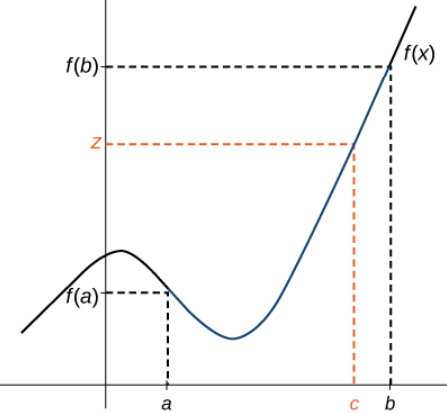
\includegraphics[scale=1]{images/Figure 2.3.2.png} 
\end{center}

Let's break down the different pieces of the theorem to better understand what it is saying. First we need to have a function which is continuous on some open interval. This does not mean that the function is only continuous on that interval, just that for the theorem to work it should be continuous on the two endpoints and everywhere in between.

For instance if we had $f(x) = 1/x$, then $[1,2]$ is a totally fine interval but $(0,2]$ is not because $1/x$ is not continuous at $x = 0$. If we had a function that is continuous everywhere like $x$ or $\cos(x)$, then any interval we pick will automatically work.

The next part of the theorem says to take some $y$-value in between $f(a)$ and $f(b)$, call it $z$. The two endpoints on the $x$-axis gives us two ``heights:" the function evaluated there. We can choose any point in that vertical range and give it a special name ($c$ in this case), this is our special little $y$-value. Keep it close to your heart.

Now the important part of the theorem. Our little $y$-value is lost, we don't know where it came from; specifically the $x$-value that got us that $y$. Unfortunately, we won't be able to find that $x$ value using the theorem, but we can at least be certain it exists and our $y$-value actually has a home it came from. The theorem tells us that there must be an $x$-value, let's call it $c$, in between the two endpoints we specified which gives us $z$. In math terms, we can apply the function to get back to our $y$ value: $f(c) = z$.

Intuitively the theorem should mostly make sense if you think long and hard about it. If we have an interval on the $x$-axis, there is another interval on the $y$-axis (see the picture above). Then since the function is continuous, if you trace the function over your interval, you must cover that $y$-axis interval at some point. There is no way around this, the only way is if you cheated and lifted your pencil in which case the function is obviously no longer continuous.

Let's see an example of this theorem in action.
\begin{example}
	Show that $f(x) = x - \sin(x)$ has at least one zero (i.e. at least one $x$-intercept). 
	
	First we note that $f(x)$ is continuous everywhere, so any interval will satisfy the first part of the theorem. We need to find two specific endpoints, one where $f(x) < 0$ and one where $f(x) > 0$. Here's two
	\[ f(-\pi) = -\pi - sin(-\pi) = -\pi < 0 \qquad f(\pi) = \pi - \sin(\pi) = \pi > 0 \]
	
	Thus the intermediate value theorem tells us there is a point, let's call it $c$, in between $-\pi$ and $\pi$ such that $f(c) = 0$. $c$ is the $x$-intercept we are looking for.
\end{example}

\newpage 
\subsection{Hard Topic: Precise Definition of a Limit}
\bigskip
\begin{mdframed}[linewidth=1pt]
CAUTION: This is a hard topic and will not be covered on the AP exam, in fact it is only lightly touched on in a normal college calculus class. This section is completely optional, proceed at your own risk and sanity.
\end{mdframed}



% Introduction to epsilon delta
% Examples
% Proving a limit law
% Very hard example/proof